%
% The standard LaTeX article class is close to what is needed for an MPhys project report
\documentclass[12pt]{article}

% The following package makes the necessary tweaks to comply with the formatting requirements.
% It also provides a standardised title page, and will warn you if the main text is too long.
\usepackage{mphysproject}
%
%% DO NOT GO CHANGING THE FONT SIZE OR MARGINS! If your main text doesn't fit within 50 pages,
%% you will have to cut stuff out.
%
%% REMEMBER: The target length is around 35 pages
%

% The formatting of the document can be enhanced by loading extra packages.
%
% An essential package is `graphicx', which is loaded by the mphysproject package so you don't
% need to load this yourself. This allows you to include figures using the \includegraphics command.
% To get more information about a package, type texdoc <package> on the Unix command line,
% substituting <package> with the name of the package, e.g., texdoc graphicx
%
% For a wider variety of mathematical environments, symbols and formatting options:
\usepackage{amsmath,amssymb}
%
% If you want to use colour in the text
%\usepackage{color}
%
% If you want to put figures side by side with separate captions
%\usepackage{subfigure}
\usepackage{subcaption}
%
% If you happen to dislike the standard TeX fonts
%\usepackage{times}
%
% If you include any URLs in your text and/or want to make cross-references clickable, include one of the following
% two lines
\usepackage{hyperref}  % This enables hyperlinks but leaves them in black, which is best for printing
%\usepackage[colorlinks=true]{hyperref} % This colours the hyperlinks, which is better for screen reading

\usepackage{csquotes}
\usepackage{braket}

\begin{document}

\title{Computing P-T Diagrams from First Principles} % Place your project title in here
\author{Max Tyler} % Put your name here
\supervisor{Dr M. Martinez-Canales} % Place your principal supervisor here
%\supervisor{Dr A. Smith} % If you have additional supervisors, list them with separate \supervisor commands
%\date{1st January 2018} % Today's date will appear on the title page by default, but if you want to tie this to a particular date, you can do so here

% Insert your abstract below
\begin{abstract}
\end{abstract}

% This command is essential to make the title page appear
\maketitle

% This command introduces the Personal Statement
\personalstatement

\textit{In the Project Report, you must submit a `Personal Statement' describing your project. The Personal Statement is to help the assessors understand what the different parts of the report represent in terms of the work you actually did. Inaccuracy in or lack of a Personal Statement may hinder the assessors and therefore lead to a reduced grade, and should be a maximum of about one page.  A real example follows.}

% If you have anyone that needs to be acknowledged (e.g., anyone who provided assistance with your project work,
% provided data etc) please do so here. Delete this (or comment it out) if you have no-one to acknowledge.
\acknowledgments

\textit{Please acknowledge any assistance that you received during your MPhys project from anyone other than your supervisor. Please also disclose here any work conducted by yourself prior to the MPhys project that is relevant to the project (e.g., summer project work). Speak to your supervisor or the course organiser if you are not sure about what might be relevant to include here.}

% This command inserts a table of contents, and sets things up for the main text of your report.
% The page count starts from here. DO NOT DELETE OR DISABLE THIS COMMAND!
\maintext


\section{Introduction}

\section{Background}
\subsection{Crystal Structure}
\subsubsection{Bravais Lattice}
A Bravais lattice, $\mathcal{B}$, is a set of points infinitely repeated throughout space, with the property that the lattice looks the same viewed from any of these points. 
An $\mathbf{N}\mathrm{-dimensional}$ Bravais lattice can be generated by a set of $n$ linearly independent vectors, the lattice basis:
\begin{equation}\label{eq:lattice_basis}
	\mathcal{V} = \{\mathbf{v}_1, \mathbf{v}_2, ..., \mathbf{v}_n\}
\end{equation}
The Bravais lattice can then be found by addition of these vectors each multiplied by some integer:
\begin{equation}\label{eq:bravais_lattice}
	\mathcal{B} = \left \{\sum_{i=1}^n a_i\mathbf{v}_i \Big | a_i \in \mathbb{Z}, \mathbf{v}_i \in \mathcal{V}  \right \}
\end{equation}
\begin{figure}
	\centering
	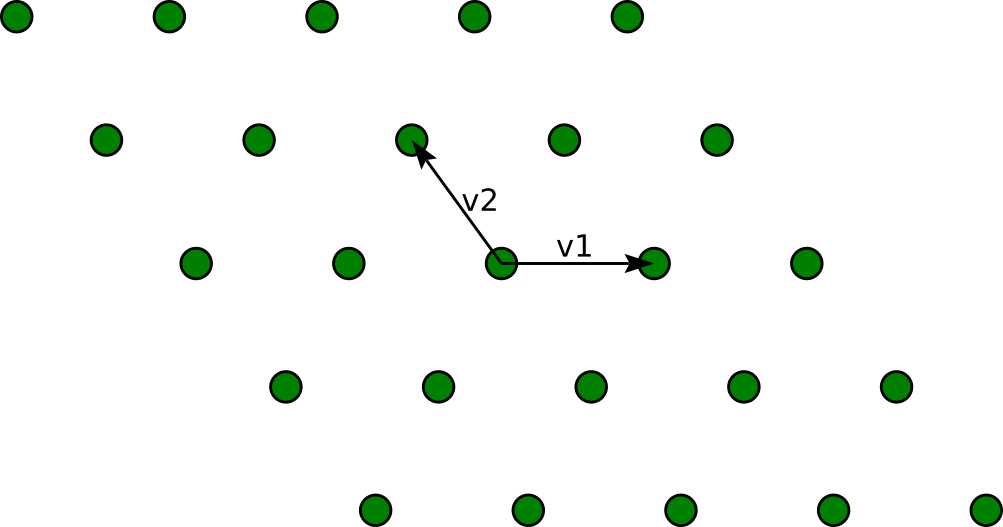
\includegraphics[width=0.6\textwidth]{./figures/lattice_basis.png}
	\caption{A 2-dimensional Bravais lattice.}
	\label{fig:lattice_basis}
\end{figure}
Figure \ref{fig:lattice_basis} shows a 2-dimensional lattice with basis vectors $\mathbf{v}_1$ and $\mathbf{v}_2$. Two Bravais lattices are considered equivalent if they are invariant under the same symmetry group. In 2 dimensions, there are 5 different Bravais lattices and in 3 dimensions, there are 14 \cite{kittel2005introduction}. The choice of a lattice basis for a certain Bravais lattice is not unique.
The Bravais lattice is invariant under translation by any of its basis vectors, meaning it is a periodic structure. 

Physical crystals also have an atomic basis consisting of a set of atoms and positions for these atoms. The atomic basis is repeated at each point on the underlying Bravais lattice and generates the physical crystal. 
A simple example is NaCl, which has a face-centred cubic Bravais lattice, and a 2 atom atomic basis (shown in figure \ref{fig:nacl_lattice}).
\begin{figure*}[t!]
    \centering
    \begin{subfigure}[t]{0.5\textwidth}
        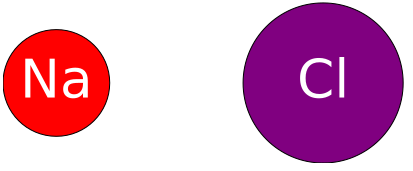
\includegraphics[width=0.7\textwidth]{./figures/na_cl_basis.png}
        \caption{The two basis atoms in NaCl}
	\label{fig:nacl_basis}
    \end{subfigure}%
    ~ 
    \begin{subfigure}[t]{0.5\textwidth}
        \centering
        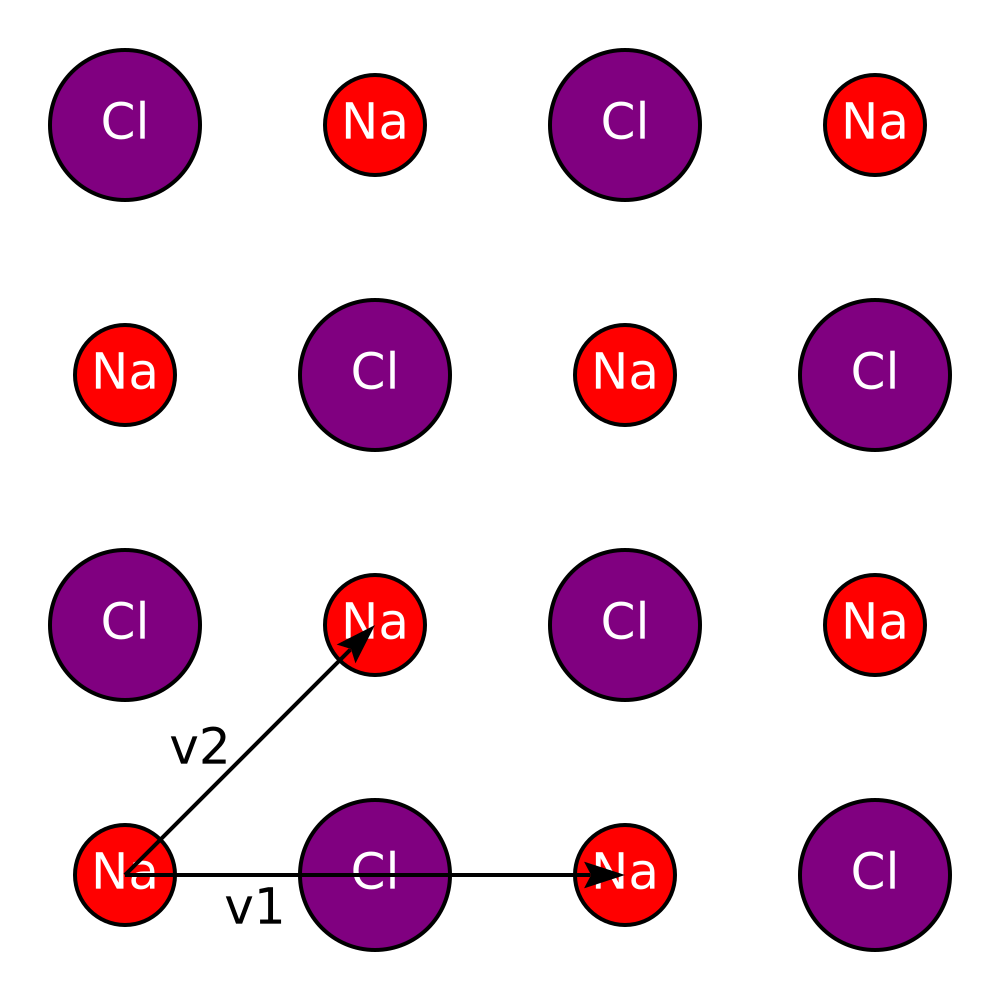
\includegraphics[width=0.6\textwidth]{./figures/na_cl_crosssection.png}
        \caption{A cross-section of the NaCl crystal, showing two of the three basis vectors}
	\label{fig:nacl_crosssection}
    \end{subfigure}
    \caption{NaCl atomic basis and crystal cross-section}
\label{fig:nacl_lattice}
\end{figure*}
\subsubsection{The Unit Cell}
The unit cell is the set of points spanned by the lattice basis vectors, and is the repeating unit that the whole crystal is tiled up from (by translating it along all lattice vectors). Specifically, it is the set of points:
\begin{equation}\label{eq:unit_cell}
	\left\{\sum _{i=1}^n a_i \mathbf v_i \Big| a_i \in \mathbb{R}, 0<a_i<1, \mathbf{v}_i \in \mathcal V \right\}
\end{equation}
The volume of the unit cell is given by the determinant of the matrix made from placing its column basis vectors together:
\begin{equation}
	V = \det [\mathbf{v}_1 \mathbf{v}_2 ... \mathbf{v}_n]
\end{equation}
\subsubsection{Dual Lattice}
With every real lattice, we can associate a dual lattice in reciprocal space with basis vectors:
\begin{equation}\label{eq:dual_basis}
	\mathcal{W} = \{\vec{\omega}_1, \vec \omega _2, ..., \vec{\omega}_n\}
\end{equation}
And a set of dual lattice points:
\begin{equation}\label{eq:dual_lattice}
	\mathcal{G} = \left \{\sum_{i=1}^n a_i\vec{\omega}_i \Big | a_i \in \mathbb{Z}, \vec{\omega}_i \in \mathcal{W}  \right \}
\end{equation}
The real and dual bases have the property:
\begin{equation}
	\mathbf v _ i \cdot \vec\omega_j = 2\pi\delta_{ij}
\end{equation}
Due to the fact that the Bravais lattice is periodic, any observable will be periodic as well (For example, the electron density, $\rho(\mathbf{r})$\ ).

Since these observables will be periodic we have:
\begin{equation}\label{eq:periodic_observable}
	f(\mathbf r) = f(\mathbf r + \mathbf B) \text{ where } \mathbf B \in \mathcal B
\end{equation}
We can consider the fourier expansion of this function:
\begin{equation}\label{eq:f_fourier_expansion}
	f(\mathbf r + \mathbf B) = \sum_k f_k e ^ {i \mathbf G_k\cdot(\mathbf r + \mathbf B)} 
	= \sum _k f_k e ^ {i \mathbf G_k \cdot \mathbf r} e ^ {i \mathbf G_k \cdot \mathbf B}
\end{equation}
Where $\mathbf G_k \in \mathcal G$, $\sum_k$ is the sum over all vectors in $\mathcal G$ and the fourier component $f_k$ is given by:
\begin{equation}
	f_k = \frac{1}{V}\int_Cd\mathbf rf(\mathbf r)e^{-i\mathbf G_k\cdot \mathbf r}
\end{equation}
$C$ being the unit cell, and $V$ its volume.

Since equation \ref{eq:f_fourier_expansion} is true for $\mathbf{B} = \mathbf{0}$, this must mean that $e^{i\mathbf G_k\cdot \mathbf B_n} = 1$, $\forall k, n \in \mathbb{Z} $ and we have that $\mathbf G_k \cdot \mathbf B_n = 2\pi N$, $N\in \mathbb{Z}$. We can generate the dual lattice vectors from the real lattice vectors (using column-vectors for the real basis and row-vectors for the dual basis): 
\begin{gather}
	\vec{\omega}_i\cdot \mathbf{v}_j = 2\pi\delta_{ij} \\
	\begin{bmatrix} 
		\vec{\omega}_1 \\
		\vec{\omega}_2 \\
		\vdots \\
		\vec{\omega}_n \\
	\end{bmatrix}
	\begin{bmatrix}
		\mathbf{v}_1
		\mathbf{v}_2
		...
		\mathbf{v}_n
	\end{bmatrix} = 2\pi
	\begin{bmatrix}
		1 & 0  & ... & 0 \\
		0 & 1 &  ... & 0  \\
		\vdots & \vdots & \ddots & \vdots \\
		0 & 0 & \hdots & 1 
	\end{bmatrix}
	\\
	\begin{bmatrix} 
		\vec{\omega}_1 \\
		\vec{\omega}_2 \\
		\vdots \\
		\vec{\omega}_n \\
	\end{bmatrix}
	= 2\pi
	\begin{bmatrix}
		\mathbf{v}_1
		\mathbf{v}_2
		...
		\mathbf{v}_n
	\end{bmatrix} ^{-1}
\end{gather}
Since the lattices are related to each other through a fourier transform, the dual lattice to the dual lattice is the original lattice.
In 3 dimensions, the reciprocal lattice of the simple cubic lattice is the simple cubic lattice 
(with each vector having a reciprocal length), the reciprocal lattice of the FCC lattice is BCC, and vice versa.
\subsubsection{Bloch's Theorem}
The periodicity of the lattice leads to a constraint on the wavefunction of electrons in the crystal:
\begin{equation}\label{eq:bloch_wave}
	\psi_\mathbf k(\mathbf r) = e^{i\mathbf{k}\cdot \mathbf{r}}u_\mathbf k(\mathbf r)
\end{equation}
Where $u_\mathbf k(\mathbf r)$ has the same period as the crystal the wave is in.
We can prove this using the translation operator $\hat T_\mathbf B$ where $\hat T_\mathbf B f(\mathbf r) = f(\mathbf r + \mathbf B)$, and $\mathbf B$ is some lattice vector. Let $\psi_\mathbf k(\mathbf r)$ be an eigenstate of the translation operator:
\begin{equation}
	\hat T_\mathbf B \psi_\mathbf k(\mathbf r) = A \psi_\mathbf k(\mathbf r)
\end{equation}
Since the state is normalised to unity, we can write $A=e^{i\mathbf k \cdot \mathbf B}$. If we define another function, $u_\mathbf k(\mathbf r) = e^{-i\mathbf k \cdot \mathbf r}\psi_\mathbf k(\mathbf r)$ and then operate on it with the lattice translation operator:
\begin{equation}\label{eq:bloch_proof}
\hat T_\mathbf B u_\mathbf k(\mathbf r) = u_\mathbf k(\mathbf r + \mathbf B) = 
e^{-i\mathbf k \cdot \mathbf r}e^{-i\mathbf k \cdot \mathbf B} \psi_\mathbf k(\mathbf r + \mathbf B) = 
e^{-i\mathbf k \cdot \mathbf r}e^{i\mathbf k \cdot (\mathbf B - \mathbf B)} \psi_\mathbf k(\mathbf r) = u_\mathbf k(\mathbf r)
\end{equation}
Which shows that $u_\mathbf k(\mathbf r)$ has the same periodicity as the lattice. The relation $u_\mathbf k(\mathbf r) = e^{-i \mathbf k \cdot \mathbf r}\psi_\mathbf k(\mathbf r)$ is then inverted to get the result in equation \ref{eq:bloch_wave}.
\subsubsection{Electrons in the Lattice}
\subsubsection{Phonons}
\subsection{Density Functional Theory}
\subsubsection{The Hohenberg-Kohn Theorems}
The Hohenberg-Kohn theorems are two theorems which make density functional theory possible. They are stated as \cite{martin_2004}:
\begin{displayquote}
	\textbf{Theorem I}: For any system of interacting particles in an external potential $v_\mathrm{ext}(\mathbf r)$, the potential $v_\mathrm{ext}(\mathbf r)$ is determined uniquely, except for a constant, by the ground state particle density $n_0(\mathbf{r})$.
\\
	\textbf{Theorem II}: A \textit{universal functional} for the energy $E[n]$ in terms of the density $n(\mathbf r)$ can be defined, valid for any external potential $v_\mathrm{ext}(\mathbf r)$.
For any particular $V_\mathrm{ext}(\mathbf r)$, the exact ground state energy of the system is the global minimum value of this functional, and the density $n(\mathbf r)$ that minimises the functional is the exact ground state density $n_0(\mathbf r)$.
\end{displayquote}
The proofs to these theorems are relatively simple, making use of the quantum variational principle \cite{shankar2012principles}. We need to make a restriction though, that the ground state of the hamiltonians in the proofs are non-degenerate.
To prove the first theorem, we use proof by contradiction with two different hamiltonians $\hat H_1, \hat H_2$ with ground state wavefunctions $\ket{\psi_1}, \ket{\psi_2}$ which give the respective ground state energies $E^0_n=\braket{\psi_n | \hat H_n | \psi_n}$. 
The hamiltonians can be separated into:
\begin{equation}
\hat H_n = \hat F + \hat V_{n, \mathrm{ext}}
\end{equation}
Where $\hat F$ contains the electron kinetic energy operator, and the electron-electron interaction operator, and is the same for the different hamiltonians. The potential operator $\hat V_{n, \mathrm{ext}}$ contains the information of the external potential on the electrons (caused by the nuclei, and maybe other factors).
We then pose that the two different potentials in the hamiltonians give rise to the same ground-state electronic density $n_0(\mathbf r)$.
The energy of the system can also be written as a functional of the electron density as:
\begin{equation}\label{eq:energy_functional}
E[n(\mathbf r)] = F[n(\mathbf r)]+ \int n(\mathbf r)v_{\mathrm{ext}}(\mathbf r)d\mathbf r
\end{equation}
Where $F[n(\mathbf r)]$ contains the electron kinetic energy and the electron-electron interaction energy, and $v_{\mathrm{ext}}(\mathbf r)$ is the external potential.
Using the variational principle, we have:
\begin{equation} 
	E^0_1 < \braket{\psi_2 | \hat H_1 | \psi_2} = \braket{\psi_2 | \hat H_2 | \psi_2} + \braket{\psi_2 |\hat H_1 - \hat H_2 |\psi_2}
\end{equation}
Using the energy functional from equation \ref{eq:energy_functional}, we can rewrite this as:
\begin{equation}\label{eq:contra_1}
E^0_1 - E^0_2 < \int n_0(\mathbf r)(v_{1,\mathrm{ext}}(\mathbf r)-v_{2,\mathrm{ext}}(\mathbf r)) d\mathbf r
\end{equation}
Swapping the indices, and rearranging gives:
\begin{equation}
E^0_1 - E^0_2 > \int n_0(\mathbf r)(v_{1,\mathrm{ext}}(\mathbf r)-v_{2,\mathrm{ext}}(\mathbf r)) d\mathbf r
\end{equation}
These equations are in contradiction with each other, and therefore, up to an additive constant, the external potential must be determined uniquely by the ground state electron density and vice versa.

To prove the second theorem, we use an energy functional $E[n(\mathbf r)]$, with some external potential $v_{\mathrm{ext}}$ that is minimised by a density $n_1(\mathbf r)$ and we consider some different density $n_2(\mathbf r)$. 
By the first theorem, the wavefunctions determined by these densities must be different ($\ket{\psi_1}, \ket{\psi_2}$) and so, using the variational principle we have:
\begin{equation}\label{eq:hk_2}
E_1 = \braket{\psi_1 | \hat H _1 | \psi_1} < \braket{\psi_2 | \hat H _1 | \psi_2} = E_2
\end{equation}
So the energy functional is minimised by this ground state density.
\subsubsection{Constrained Search}
\subsubsection{Density Functional Perturbation Theory}

\section{Methods}


\section{Results and Discussion}

\section{Conclusion}

\section{References}

% This command tells LaTeX how to format your references in the biblography. The standard plain formatting, with
% references appearing in the order they are cited, is absolutely fine for our needs.
\bibliographystyle{unsrt}

% This command includes the reference list. You will need to compile two or three times (perhaps BiBTeXing after
% the first time) to get the references in synch with the text.
\bibliography{ref}

% This command switches to appendices. The page count ends here.
% NOTE: the material contained in appendices will NOT count towards the assessment of your report.
% Consequently the main text should be self-contained.
\appendix

\end{document}
